\section{Introduction}
\label{sec:introduction}

% state the learning objective 
The objective of this laboratory assignment is to study a stationary circuit containing two
voltage sources $V_a$, independent, and $V_c$, dependent, two current sources, $I_d$, independent and $I_b$, dependent, and resistors, as shown in Figure~\ref{fig:rc}.


In Section~\ref{sec:analysis}, a theoretical analysis of the circuit is
presented, based on mesh and nodal methods. In Section~\ref{sec:simulation}, the circuit is analysed by
simulation, and the results are compared to the one presented before in Section~\ref{sec:analysis}. The conclusions of this study are outlined in
Section~\ref{sec:conclusion}.

\begin{figure}[h] \centering
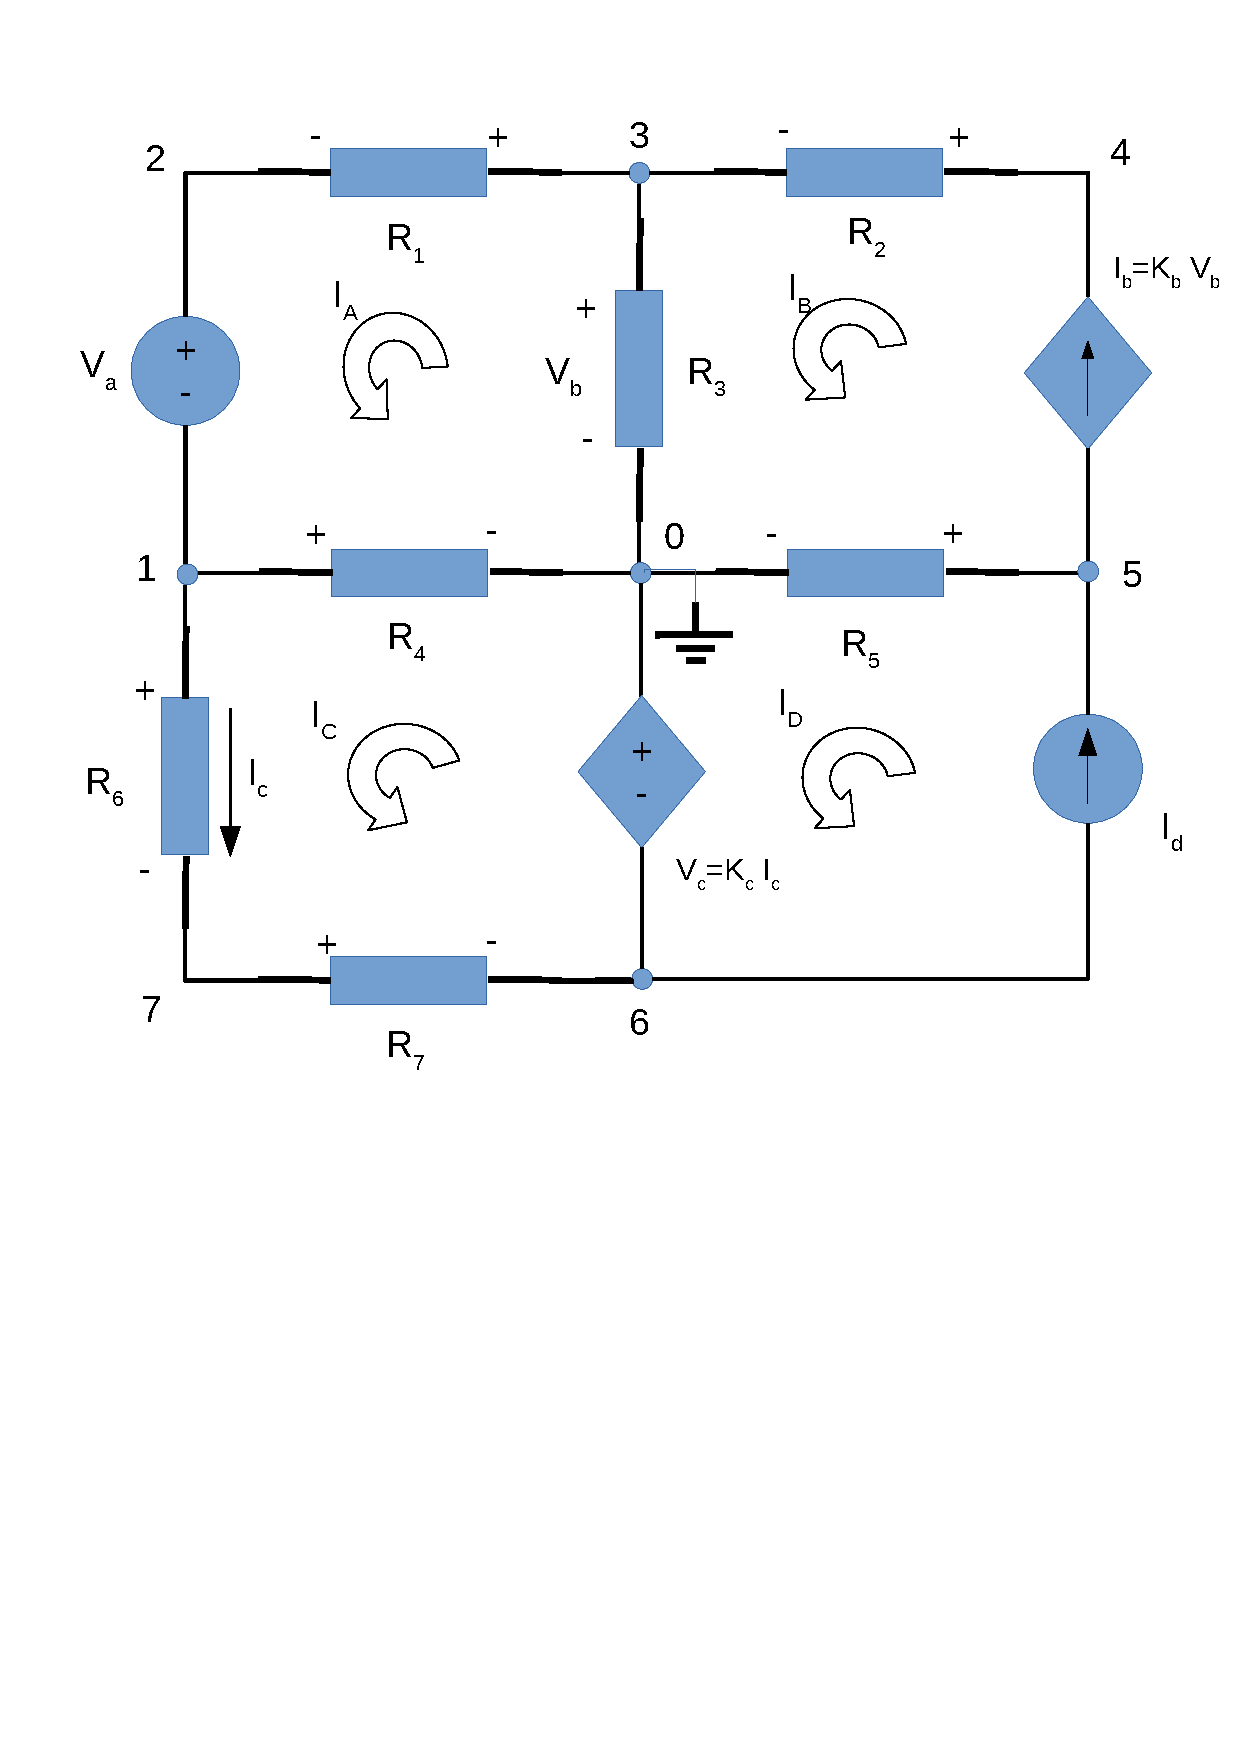
\includegraphics[width=0.4\linewidth]{circuito1.pdf}
\caption{Studied Circuit.}
\label{fig:rc}
\end{figure}

